\section[Introduction: input based measure]{An input based information measure for adaptive controllers \label{Chapter5:Max Corr Input}}

This Section describes the development of an information measure
to assess the learning performance of the, previously described, learning agents
in the social system.

Therefore the main purpose of this Section is to introduce a couple of correlation 
based performance measures which are computed at the sensory inputs of the agent.
The first measure is called \textbf{maxcorr}, is very simple and
can be computed in real time without any probability estimation.
The \textbf{maxcorr} measure can then be normalised by using a logarithmic approach
to express the learning performance in terms of bits and thus is called \textbf{AI measure} .
The simplicity of the AI measure derives from the dependency on the
representation used by the controller/agent, but it has the disadvantage of
not being general, as described in the discussion.

\subsection{Introduction to the maxcorr input measure}
This section describes an information measure suitable for closed loop
controllers that makes use of temporal unsupervised learning. It can be applied
for example to ICO/ISO learning, differential and temporal Hebbian learning.
This information measure estimates how much the agent/controller has learnt
and is directly correlated to the weight change of the learning rule used.
The measure is based on the agent's perspective (at the input side) rather
than at output side as previous approaches. Looking at the output is equivalent
 to analysing behaviour and has a disadvantage: agents adapt to the complexity
of the environment thus even a simple reactive agent has increasing complex
behaviour in an increasingly complex environment \citep{NolfiInteraction}.
As I argued before in the previous Section \ref{Introduction:InfoTheoryClosedLoop}, 
organisms perform input control because
neural activity (motor output) generates other neural activity (sensory input) and 
so it is clear that an input measure can capture the performance of any agent, especially
 the one that are based on ICO/ISO controllers which performs input correlation.
Input                                                                                                                                                                                                                                                                                                                                                                                                                                                                                                                                                                                                                                                                                                                                                                                                               control is a closed loop property and is agent centric, whereas output control is 
observer centric. 
To my best knowledge, this is the first approach for the closed loop case,
which is not based on the traditional concept of Shannon's entropy.
In this model agents are learning to avoid obstacles and each other using a proximal signal
(touch sensor as pain) and a predictive signal (vision). An information
measure is computed on these inputs to verify if the agents are learning.
Firstly the author introduces the information measure based on the cross correlation
of the agent inputs, then he applies the measure to two types of agent controllers (a complex and a simplified model)
for an avoidance task with multiple agents.
Finally the measure is computed on the social setting described in section \ref{Chapter4:Social adaptation}.

\subsection{Methods: controller assumptions}
The following assumptions were made for the development of the measure:
\begin{itemize}
\item the controller is a MIMO (multi input multi output) or MISO (multi input single output)
\item input signals can be analog or digital
\end{itemize}

The closed loop measure is based on the cross correlation to be applied to the
input signals (minimum is 2) of the adaptive controller.
Cross correlation of two real analog signals $x(t),y(t)$ of a real variable $t$
(in our case time), denoted as $corr(x,y)$ is defined by:
\begin{equation}
corr(x,y)=\int_{-\infty}^\infty x(\tau)\,y(t+\tau)d\tau.
\end{equation}
Cross correlation for realisable devices (software or hardware implementations)
must be computed in finite time, that means computing the cross correlation
in a limited time window $T<\infty$:
\begin{equation}
corr(x,y)=\int_{t}^{t+T} x(\tau)\,y(t+\tau)d\tau.
\end{equation}
Cross correlation for digital signals (sampled analog signals) as two discrete
time series $x_{n},y_{n}$ with $n=1,..,N$ is defined as:
 \begin{eqnarray}
 R_{xy}(m)=\sum_{n=0}^{N-m-1}x_{n+m}y_{n} & m \geq 0 \\
 R_{yx}(-m)=0 & m <0\\
 c_{xy}(m)=R_{xy}(m-N) & m=1,2,...,2N-1\label{eq:xcorrdigital}
\end{eqnarray}

The cross correlation give us a measure of the linear synchronisation between x and y.
Its absolute values range from zero (no synchronisation) to 1 (maximum synchronisation)
and it is symmetric: $c_{xy}(m)=c_{yx}(m)$. Peaks in the cross correlation determine
the phase delay between signals (for other cross-correlation variation see \ref{Appendix:crosscorr}).

The next section describes a complex model for an avoiding robot using the ICO
learning rule.

\subsection{Methods: complex model configuration}
The simulation model is composed of a 2 dimensional world bounded by walls
as described before in Chapter \ref{WorldModelSim}.
The agents are indexed by their position as $a_{j}(t)$, where $a_{j}$
has 2 components (x,y coordinates indexed by $a_{j,x}$ and $a_{j,y}$),
with $j=1,..,N$. Agents move with a differential drive system (two wheels).

In this configuration the agent has only an avoidance behaviour:
\begin{itemize}
\item left and right reflexes makes him retract when both synapses are active
\item left and right distals are being used later on when the agent has learned
the association of distal to reflexes.
\end{itemize}

Agents and walls are obstacles. Agents produce obstacle signals.
Every agent $a_{j}(t)$ has a potential field associated (see Eq.\ref{eq:circle}):
\begin{equation}
Gavoid_{j}(t)=G(x-a_{j,x}(t),y-a_{j,y}(t)).
\end{equation}
that is sensed by the corresponding inputs of other agents $a_{k}(t)$
(with $k\neq j$) labelled as $avoid_{left,right}$. Walls
don't produce $G_{avoid}$, so that agents sense them using proximal signals that are
generated by collisions: when 2 distinct agents $j$ and $l$ collide at time $t_{0}$, such
that $||a_{j}(t)-a_{l}(t)||_{2}<D$ ($D$ is the radius of the
agent) an impulse is produced an impulse is produced at $avoid_{l,r}$.
\begin{figure}[htb]
\begin{center}
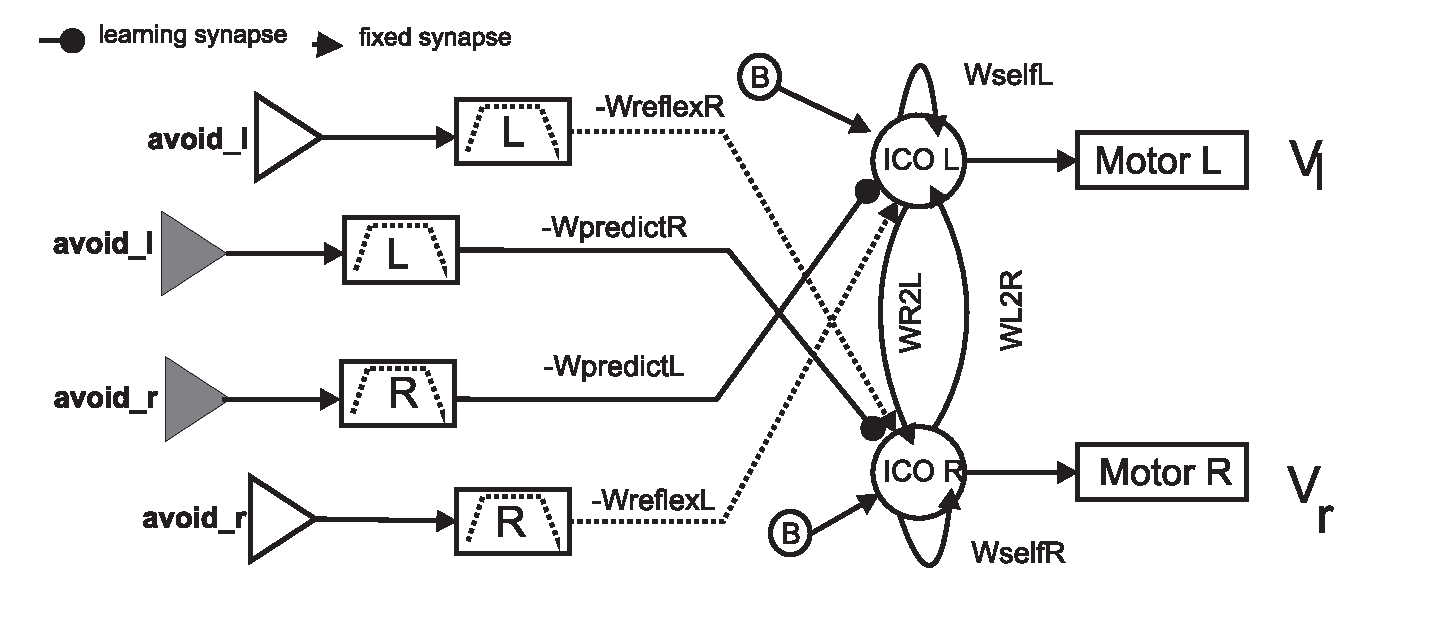
\includegraphics[scale=0.45]{figures/infomeasure/avoidance.eps}
\end{center}
\vspace*{4pt}
\small{
\caption[Avoidance ICO behaviour]{
Avoidance network: ICO left and right are two neurons implementing the
ICO learning rule, their output is a sigmoid and is connected (after
normalisation into $[v_{min},v_{max}]$) to the motor speed commands.
Grey triangles represent distal inputs, while white triangles represent
proximal inputs. The learned synaptic weights are associated to the distal
synapses (thick lines) while the fixed are associated to the proximal synapses
(dotted lines). To produce a retraction behaviour left and right weights
must be different such that
$W_{predict,L}>W_{predict,R}$ and $W_{reflex,L}>W_{reflex,R}$, if
$W_{predict,L}=W_{predict,R}$ and $W_{reflex,L}=W_{reflex,R}$ robot
will just go back without turning.\label{fig:inputcorr:avoidance}}}
\end{figure}
The agent's controller, (shown in Fig. \ref{fig:inputcorr:avoidance}) is composed of:
\begin{itemize}
\item two input synapses: left and right with one reflex and one distal signal per synapse.
\item two ICO neurons: left and right cross connected as left synapse with right motor and right synapse to the left motor.
\item two output motors: respectively for the left and right ICO neuron connected to the left and right motor speed.
\end{itemize}

Every ICO neuron (left and right) has 2 corresponding reflexes
(left, right short range sensors) connected:
\begin{eqnarray}
x_{0,l}(t)=avoid_{prox,r}(t) & x_{0,r}(t)=avoid_{prox,l}(t)
\end{eqnarray}
and 2 corresponding predictive signals (left, right long range sensors) connected:
\begin{eqnarray}
x_{1,l}(t)=avoid_{dist,r,d_{o}}(t) & x_{1,r}(t)=avoid_{dist,l,d_{o}}(t).
\end{eqnarray}

The neural controller for the avoidance behaviour is shown in
Fig. \ref{fig:avoidance} \citep{Stamm2006}, every ICO neuron (left and right)
computes the following operations:

\begin{eqnarray}
ICO_{L}(t)&=B-h \ast x_{0,r} \cdot W_{reflexL}-h \ast x_{1,r}\cdot W_{predictL}\\ \nonumber
	  &+W_{selfL}\cdot ICO_{L}(t-1) + W_{L2R}\cdot ICO_{R}(t) \label{eq:input:ICO:L1} \\ 
ICO_{R}(t)&=B-h \ast x_{0,l}\cdot W_{reflexR}-h \ast x_{1,l}\cdot W_{predictR}\\ \nonumber
	  &+W_{selfR}\cdot ICO_{R}(t-1) + W_{R2}\cdot ICO_{L}(t)  \label{eq:input:ICO:R1}
\end{eqnarray}

The parameters used for the weights, the bias and the recurrent connections are
reported in the Appendix sections \ref{Appendix:HysteresysValue},\ref{Appendix:simulation}.
The recurrent connections between the left and right ICO neuron, are necessary
to implement a push-pull behaviour so that when the robot synchronously activates
both the left and the right input, only one ICO neuron will dominate thus evoking
a turn-back response. 
Connections between input synapses and ICO neurons (motor neurons) are
negative to evoke a retraction. 
The motor output is calculated with a sigmoid activation function on the ICO neuron
membrane as follow:

\begin{eqnarray}
V_{L}&=& \frac{1}{1+e^{-ICO_{L}}}\\
V_{R}&=& \frac{1}{1+e^{-ICO_{R}}}
\end{eqnarray}

The weight update learning rule is calculated for the weights:

\begin{eqnarray}
\frac{\partial W_{predict,L}}{\partial t}&=& \mu \cdot x_{1,l} \frac{\partial x_{0,l}}{\partial t} \label{eq:maxcorr:wleft}\\
\frac{\partial W_{predict,R}}{\partial t}&=& \mu \cdot x_{1,r} \frac{\partial x_{0,r}}{\partial t} \label{eq:maxcorr:wright}
\end{eqnarray}


\subsection{Methods: cross correlation and ICO learning}
Cross correlations are computed for the left and right synapse at fixed non
overlapped time windows $\triangle T$ expressed in seconds.
Considering Eq. \ref{eq:xcorrdigital} $N_{s}=\triangle T/\delta t$ is the number
 of samples in a time window of $\triangle T$ with a $\delta t$ as sampling time.
Left and right cross correlations are computed for every non overlapping time window $k=1,2,...$
\begin{eqnarray}
xcorr_{left}(k)=corr(H(x_{1,l}),H(x_{0,l}))=corr(u_{1,l},u_{0,l})\\
xcorr_{right}(k)=corr(H(x_{1,r}),H(x_{0,r}))=corr(u_{1,r},u_{0,r})
\end{eqnarray}
where $k$ is the index of the time window where the cross correlation was computed,
$H$ is a high pass filter that removes the constant component (generally referred as $DC$)
from the cross correlation diagram. Removing the $DC$ bias is necessary for the application
of statistical measures (see Appendix \ref{Appendix:crosscorr}).
In our model the high pass filter $H$ because the inputs of my artificial agents 
are receiving only discrete events, so essentially impulses with a 0 bias as in figure \ref{fig:ico}.
For every time window $k$, I computed the maximum $max$, energy $E$,power $P$ of the
left $xcorr_{left}(m,k)$ and right $xcorr_{right}(m,k)$ cross correlation plus the average of
the weight change for left and right $W_{predict,L},W_{predict,R}$.
\begin{eqnarray}
M(xcorr_{left}(k))=& \max\limits_{m}(xcorr_{left}(m,k)) \label{eq.maxcorr:mleft}\\
M(xcorr_{right}(k))=& \max\limits_{m}(xcorr_{right}(m,k)) \label{eq.maxcorr:mright}\\
E(xcorr_{left}(k))=& \sum\limits_{m} xcorr_{left}(m,k)^2  \\ 
E(xcorr_{right}(k))=& \sum\limits_{m} xcorr_{right}(m,k)^2 \\ 
P(xcorr_{left}(k))=& \frac{\sum\limits_{m} xcorr_{left}(m,k)^2}{N} \\
P(xcorr_{right}(k))=& \frac{\sum\limits_{m} xcorr_{right}(m,k)^2}{N} \\
Avg(W_{predict,left},k)=&\frac{\sum\limits_{m} W_{predict,left}(m+k N_{s})}{N_{s}} \\
Avg(W_{predict,right},k)=& \frac{\sum\limits_{m} W_{predict,right}(m+k N_{s})}{N_{s}} \\ 
\end{eqnarray}
The reason why I have computed this values for the left and right synapse is that
these weights develop independently from each other as in Eq. \ref{eq:maxcorr:wleft},\ref{eq:maxcorr:wright}.
Since energy and power are related measures only energy is computed (see Appendix \ref{app:energy}).
The average of the weight change for the left and right distal synapses is computed
 to validate the information measure for the result section.

\subsection{Methods: a simplified model}
The agent controller can be over simplified by using only one weight and thus one
ICO controller for the avoidance behaviour.
The difference between the left and right far antennas provides $x_{1}$ and the
difference between the left and right near short antennas provides $x_0$.
The band pass filters in Fig.\ref{maxcorr:methods:ico1} generate $u_{0},u_{1}$
that are damped waves if $x_0,x_1$ are delta pulses.
The transfer function of the band pass filter is specified in the Laplace-domain as:
\begin{eqnarray}
h(t)& &\leftrightarrow H(s) =\frac{1}{(s+p)(s+p*)}\\
h(t)&=&\frac{1}{b}e^{at}sin(bt)\\
a &=&-\pi \frac{f}{q}\\
b &=&\sqrt{(2\pi f)^2 -a^{2}}
\end{eqnarray}
where $p*$ represents the complex conjugate of the pole $p = a + ib$, $f$ is the
oscillation frequency and $q$ is the quality factor of the filter.
ICO correlates the predictive signal $u_{1}$ with the reflexive signal $u_{0}$
according to the formula:
\begin{equation}
 \frac{d\omega_1}{dt}=\mu \cdot u_1 \cdot \frac{du_0}{dt}
\end{equation}
where $\omega_1$ functions now as the weights of the more complex model in Eq. \ref{eq:maxcorr:wleft},\ref{eq:maxcorr:wright}.
Then the output $z$ of the controller is used to control the steering angle of
the robot such that an obstacle on the left $u_0>0$ will produce an anticlockwise turn,
whereas an obstacle on the right $u_0<0$ will produce a clockwise turn.
The controller learns to avoid the error signal $u_{0}$ using the predictive
signal $u_{1}$. Fig.\ref{maxcorr:methods:ico1}(A) illustrates how the learning
is achieved and (B) describes how the agents interact with the world.
A purely reactive agent has only a reflexive behaviour via $u_0$ and will never
learn to avoid the loop error signal $u_{0}$: it will touch the obstacle and
produce a trajectory like (1). When the agent starts to learn ($\omega_{1}>0$)
it will use the $u_{1}$ to prevent $u_0$, thus avoiding the obstacle before touching
it like the trajectory in (2).
Figure \ref{maxcorr:methods:ico1}(C) shows how the reflex signal is shifted forward
in time and reduced in amplitude due to the anticipatory motor reaction of the controller.
\begin{figure}[!htbp]
\begin{center}
%\framebox[4.0in]{$\;$}Schematic1
%\fbox{\rule[-.5cm]{0cm}{4cm} \includegraphics[scale=0.6]{Schematic1} \rule[-.5cm]{4cm}{0cm}}
\includegraphics[width=0.6 \textwidth]{figures/infomeasure/simple/simplemodel.eps}
\end{center}
\caption[Simplified control model]{A) Schematic diagram of the closed-loop learning
 system with inputs $x_0$ and $x_1$, synaptic weights $\omega_0$ and $\omega_1$ and
 motor output $z$. $P_0$ and $P_1$ are the transfer functions of the reflexive and
 the predictive pathway. BP block is a 2 pole band pass filter. B) Agent setup with
 short range antennas (reflexive inputs, $x_0$) and long range antennas (predictive inputs, $x_1$).
The agent is learning to avoid obstacles and walls using its short and long range antennas.
The motor reaction will reduce the intensity of the painful reflex $x_0$ as well as
 delay its occurrence. C) Schematic diagram of the input correlation learning rule
 and the signal structure \citep{Porr2006ICO}. The $u_0$ and $u_1$ are respectively
 the difference between the filtered values of the left and right antennas of
the agent. During learning the $u_0$ peak will be shifted in time and reduced
 in amplitude. \label{maxcorr:methods:ico1}} 
\end{figure}

\subsection{Methods: anticipatory information}
Within the simplified model, the equations in \ref{eq.maxcorr:mleft} and \ref{eq.maxcorr:mright}
collapse in a unique value which is defined as $cc(t)$ as in Eq. \ref{eq:maxcorr:cc}.
Intuitively the information measure grows when the agent is using anticipatory information
and is zero when the agent is not able to predict its reflex.
Before learning the predictive signal $u_1$ is followed always by the reflex signal $u_0$
with the same amplitude, while after learning the amplitude of $u_0$ is likely reduced.
An ideal learner will be able to reduce totally the reflex $u_0$ to 0.
One will also notice that generally, after learning, the reflex $u_0$ will not only
be reduced but also delayed in time.

\begin{figure}[htbp]
\begin{center}
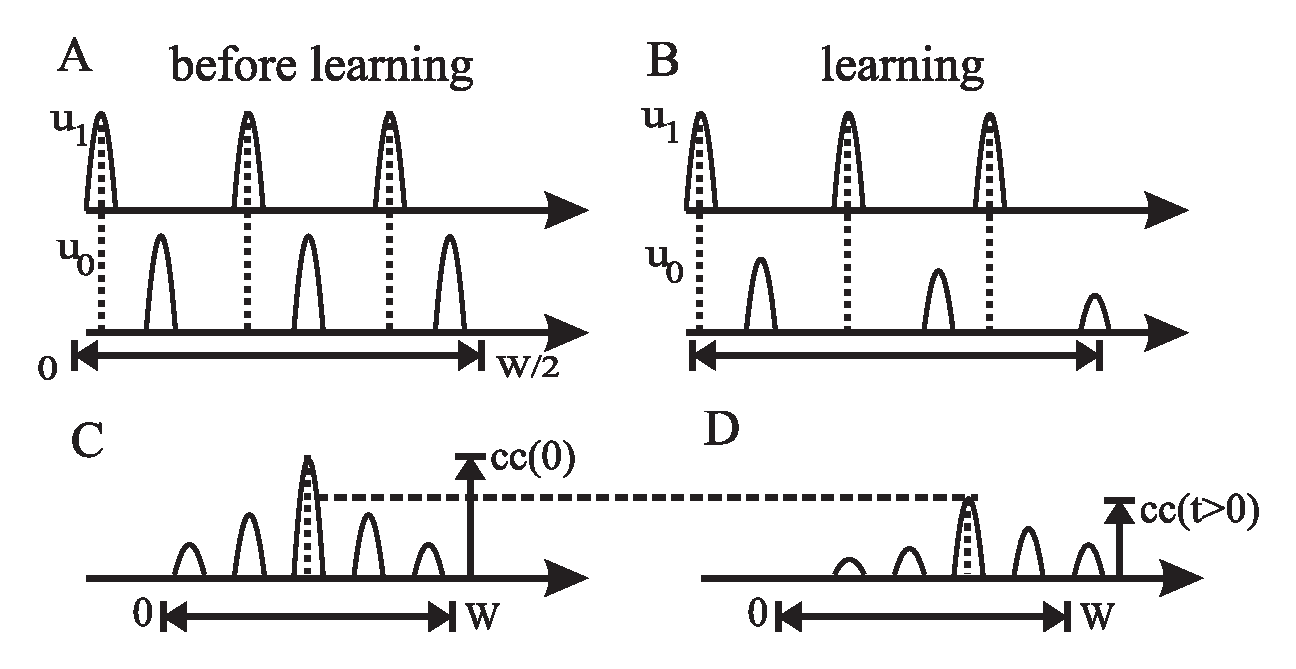
\includegraphics[width=0.6 \textwidth]{figures/infomeasure/simple/temporalsignal.eps}
\end{center}
\begin{small}
\caption[Temporal signal development during learning]{A) Illustration of the signals $u_1,u_0$
of a non learning agent. The peaks are periodic but off phase and with same amplitude.
B) Same time diagram for a learning agent. C) Cross correlation of $u_1$ and $u_0$ for the non learning case.
D) Cross correlation of $u_1$ and $u_0$ for the learning case. \label{methods:xcorr}}

\end{small}
\end{figure}

Fig.\ref{methods:xcorr} shows a typical temporal diagram of events for a non
learning agent A and for a learning one B.
If one takes the cross correlation between the $u_1$ and $u_0$ for both cases,
it is possible to understand by the cross correlation which agent is learning and
 which one is not. For instance the non learning agent has a cross correlation
that is not shifted in time and reduced in amplitude like in Fig.\ref{methods:xcorr}(C),
while a learning agent has a cross correlation that is shifted in time and reduced
in amplitude like in Fig.\ref{methods:xcorr}(D).
My purpose is now to quantify this performance by using an information based measure
in terms of information bits.
Therefore a normalised version of $cc(t)$,$AI$ is computed in 2 steps:
\begin{align}
cc(t)=max (\sum_{\tau=-\frac{W}{2}}^{\tau=\frac{W}{2}} u_{1}(t)\cdot u_0(t+\tau)) \label{eq:maxcorr:cc}\\
AI(t)=-log_{2}(\frac{cc(t)}{cc(0)})\\
0 \leq \frac{cc(t)}{cc(0)} \leq 1
\end{align}
$cc(t)$ is the maximum of the cross correlation between the error signal and
the predictive signal in the time window $W$ that must be sufficiently large
to take at least a pairing of $u_1$ with $u_0$ when learning is off. $cc(0)$
is the maximum of the cross correlation computed when the agent is not learning,
whereas $AI(t)$ takes the ratio between the current and the initial cross correlation,
thus the argument of the logarithm will range from 0 to 1 because the correlations
following the first one can at least be equal to the first one.
When learning is off, the agent's predictive signal precedes the reflex signal whose
amplitude is not reduced hence $AI\simeq 0$, when learning is on, the agent learns
to reduce the error $u_{0}$, using an earlier motor reaction elicited by $u_{1}$,
thus the $AI \rightarrow \infty$ in the ideal case of perfect learning.
In terms of information bit, a reduction of $cc(t)$ by half can be interpreted
as an improvement of 1 bit as discussed in the results section.
In terms of information, if the agent is learning continuously the number of bits of
the $AI$ will increase in time until the agent has completely avoided the reflex.
In the next section I go back to the complex model and compute the cross correlation
and energy for the left and right synapses.
After that I will perform a benchmark of $AI$ for a the simplified model.
Both measures are taken in a multi agent scenario to see the effects of 
multiple learning agents.
I then compute the $AI$ for the simplified model in the social system and
draw some conclusions.

\subsection{Results: complex model results}
Simulations with the complex model were executed with an increasing number of agents in a rectangular
bi-dimensional world with obstacles. 
The software used to simulate the agents is Enki \footnote{http://home.gna.org/enki/}
an open source simulator for multiple robots interacting on a flat surface.
The simulator implements collisions, physics support (like slip, friction etc..)
and features 4 realistic robots.
For our simulations I used a group of Alice robots and setup the experiment as follow:
\begin{itemize}
\item $N=2$ agents and  $M=2$ obstacles
\item $N=4$ agents and $M=2$ obstacles
\item $N=4$ agents and $M=2$ obstacles, and an introduction of an agent
\end{itemize}
Agents for every case are numbered from $0$ to $N-1$.
The world's area $A_{world}$ is proportional of a factor $K$ to the sum of the agent's area:
\begin{equation}
 A_{world}=K_{a} \cdot (\sum_{i=1}^{N} A_{agent} )+ K_{o} \cdot (\sum_{i=1}^{M} A_{obstacle} )
\end{equation}
where  $A_{world}$,$A_{agent}$,$A_{obstacle}$ are respectively the area of the world,
the area of the agent and the area of the obstacle.
This normalisation technique is necessary to provide approximately the same amount 
of sensory events when the area get more crowded.
Intuitively speaking, if I keep the same area and add an increasing amount of agents
there will be a proliferation of collision and thus reflexes as well as predictor
events and thus comparison of the measures will not be reliable.
Simulation time for every setup was set to $T_{max}=600000$ steps,
$\triangle T=600 $, with sampling time $\delta t=0.01$ seconds.
Learning is switched on $\mu >0$ for $t> \triangle T=600$:
the cross correlation of the first time window is
computed when agents are only using reflexes (reactive agents).
If I compute the measure for two purely reactive agents as in Fig. \ref{entropy:reactive},
I can see that the values are constant for the left and right synapse: the agent is not learning
anything about the causal relations of distal and proximal signal.
This is because the $u1$ event is followed always by a $u0$
with the same amplitude and thus $xcorr$ amplitude is steady as described in the 
simplified model of Figure \ref{methods:xcorr}(A,C).

\begin{figure}[ht]
  \begin{center}
    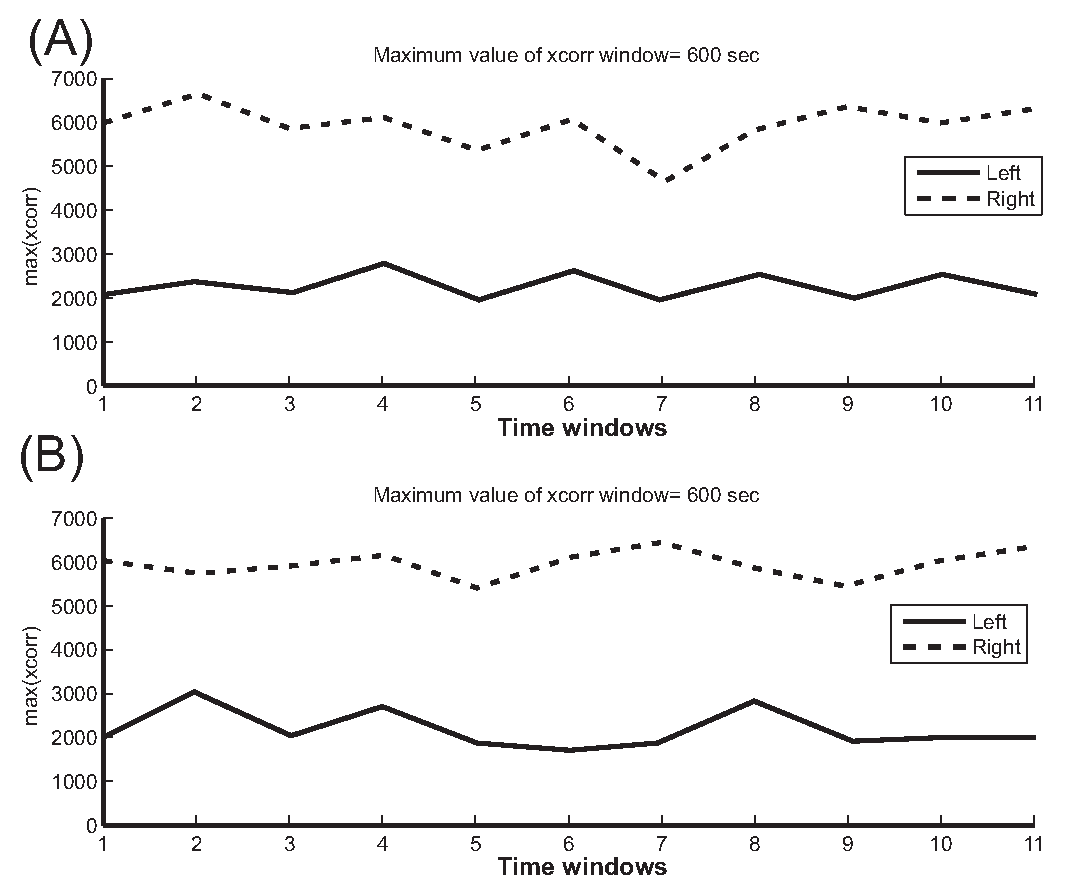
\includegraphics[scale=0.6]{figures/infomeasure/maxcorr_nolearn.eps}
    \caption[Max correlation for non learning agents]{
	     Two agents are moving in the environment without learning $\mu=0$.
	     The $M(xcorr_{left}(k)),M(xcorr_{right}(k))$ are computed for each reactive agent, A and B.
	     The measure is constant: agents are not learning anything from
	      the environment. \label{entropy:reactive}}
  \end{center}
\end{figure}
Another important property to notice in Fig. \ref{entropy:reactive} is the difference
in the offset between the $M(xcorr_{left}(k))$ left maximum cross correlation and
the $M(xcorr_{right}(k))$ right maximum cross correlation.
This is due to the initial bias of the avoiding behaviour for the agent, because 
$W_{predict,L}>W_{predict,R}$ and thus the agent tends to turn on the left each
time an obstacle is encountered.

\paragraph{Experiment with 2 agents and 2 obstacles}
Fig.\ref{fig:N2M2} shows the measures for $N=2$ learning agents and $M=2$ obstacles.
\begin{itemize}
 \item Fig.\ref{fig:N2M2}(a) contains the $M(xcorr_{left}(k))$, $M(xcorr_{right}(k))$ in the upper panel
and the $Avg(W_{predict,left},k)$, $W_{predict,right},k)$ in the lower panel for the first agent.
 \item Fig.\ref{fig:N2M2}(c) contains the $M(xcorr_{left}(k))$, $M(xcorr_{right}(k))$ in the upper panel
and the $Avg(W_{predict,left},k)$, $W_{predict,right},k)$ in the lower panel for the second agent.
\item Fig.\ref{fig:N2M2}(b) contains the $E(xcorr_{left}(k),E(xcorr_{right}(k))$ in the upper panel
and the $Avg(W_{predict,left},k)$, $W_{predict,right},k)$ in the lower panel for the first agent.
\item Fig.\ref{fig:N2M2}(d) contains the $E(xcorr_{left}(k),E(xcorr_{right}(k))$ in the upper panel
and the $Avg(W_{predict,left},k)$, $W_{predict,right},k)$ in the lower panel for the second agent.
\end{itemize}

Each agent this time is learning $\mu>0$ to avoid each other and so the weights are
decreasing $W_{predict,right},k)$ like in Fig.\ref{fig:N2M2}(a) bottom, although not equally
because the left input is stronger and does not allow the same amount of learning
on the right input.
The weight change reflects the  corresponding correlation measure Fig.\ref{fig:N2M2}(a) up,
because the cross correlation for the left $M(xcorr_{left}(k))=0$ and right $M(xcorr_{right}(k))=0$
goes to zero when the weights are stabilised, indicating that the reflex is not triggered
any more when $k>7$.

Oscillation of $M(xcorr_{left,right})$ are present because the agent is learning on average to avoid
the reflex: that means sometimes due to the complexity of the environment some
unpredictable events can still occur.
For example agent 1 can appear suddenly in the range of agent 0 which is already
avoiding another obstacle and inevitably will hit either the obstacle or the agent 1.

The energy of the signal is useful to estimate the complexity of the environment
composed by the obstacles and the other learning agents:
the more pairing of distal and proximal events the bigger the energy.
Energy is high $E(xcorr_{left}(k))$ and $E(xcorr_{right}(k))$ when all agents are unpredictable
(learning rate is not stable) $k<6$ as in Fig.\ref{fig:energy1N2M2},\ref{fig:energy2N2M2}
Indeed increasing the number of agents to $N=4$ increases the level of energy and conversely, 
decreasing the number of agents reduces the level of energy.

\begin{figure}[htbp]
  \begin{center}
      \subfigure[Cross correlation maximum $M(c_{d}(k))$ for left (straight) and right (dashed) synapses. Measures from agent 0.]{
	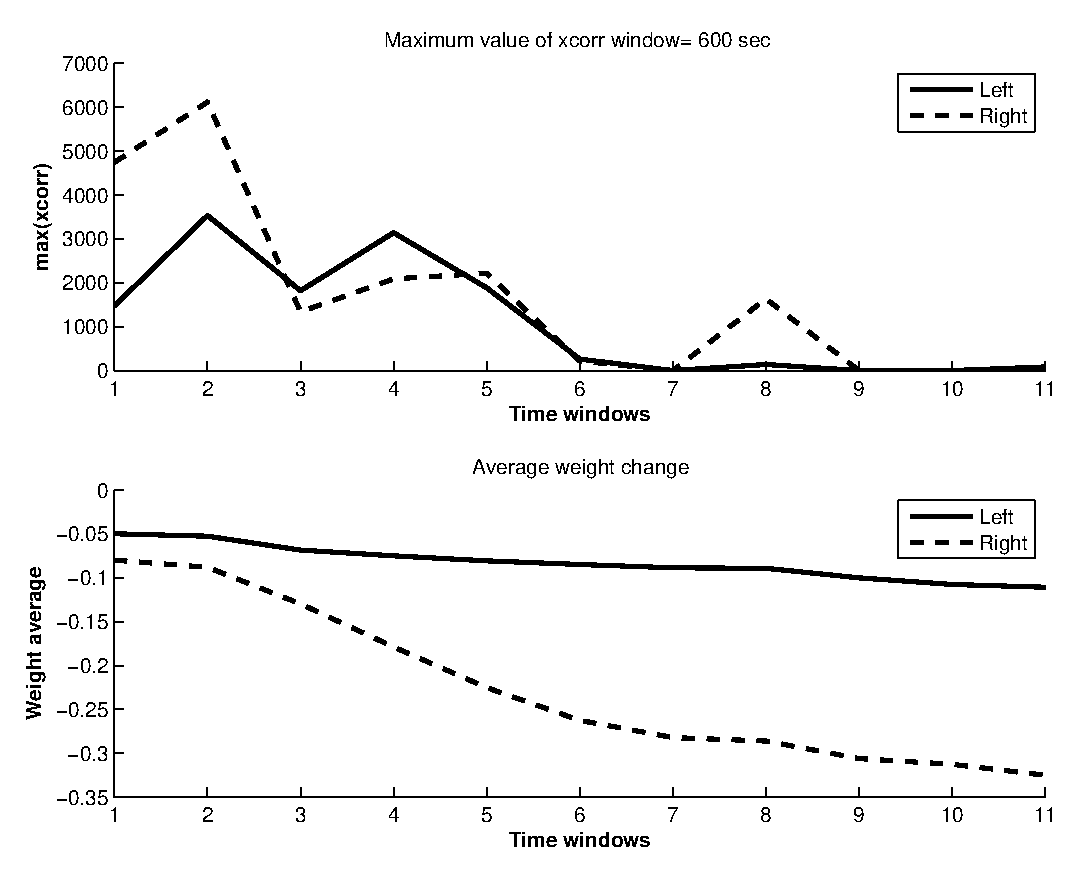
\includegraphics[scale=0.3]{figures/infomeasure/N2/maxcorr_N=0_w=600.eps}}
	\hspace{1pt}
      \subfigure[Energy $E(xcorr_{d}(k))$ for left (straight) and right (dashed) synapses. Measures from agent 0.\label{fig:energy1N2M2}]{
	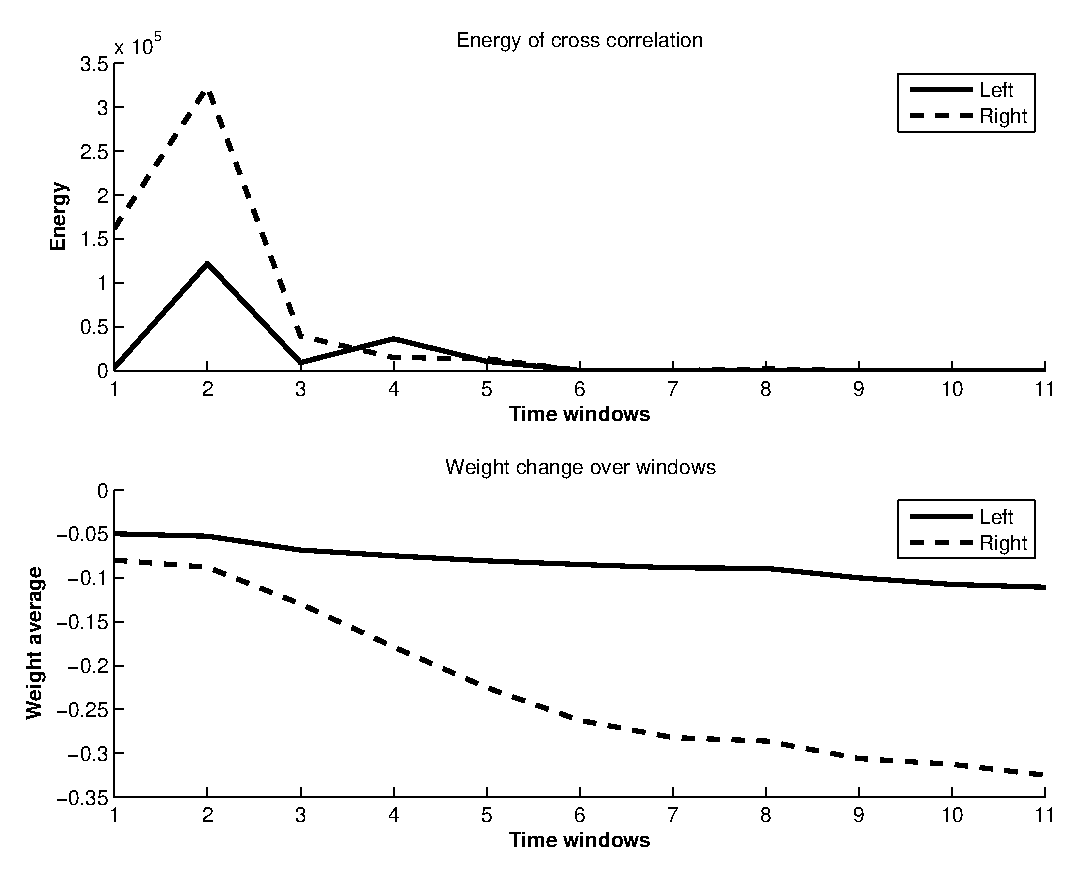
\includegraphics[scale=0.3]{figures/infomeasure/N2/power_xcorr_N=0_w=600.eps}}
      \subfigure[Cross correlation maximum $M(c_{d}(k))$ for left (straight) and right (dashed) synapses. Measures from agent 1.]{
	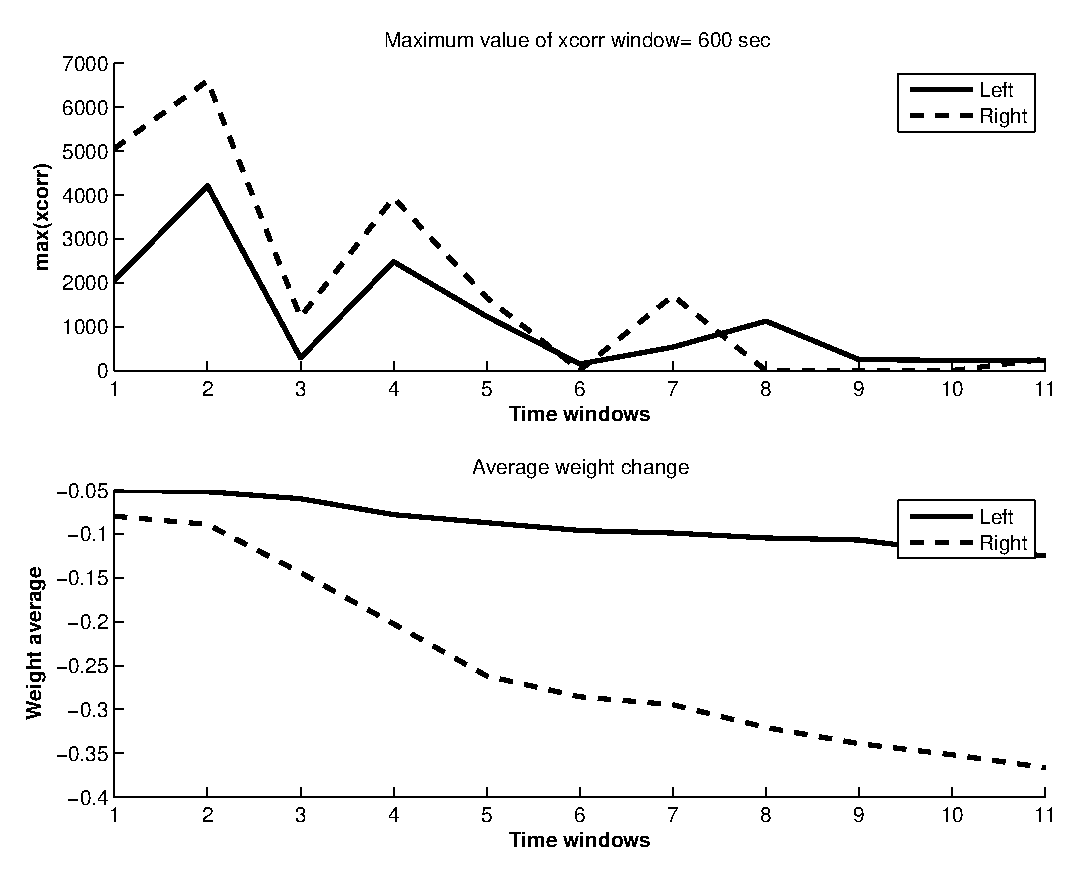
\includegraphics[scale=0.3]{figures/infomeasure/N2/maxcorr_N=1_w=600.eps}}
	\hspace{1pt}
      \subfigure[Energy $E(xcorr_{d}(k))$ for left (straight) and right (dashed) synapses. Measures from the agent 1.\label{fig:energy2N2M2}]{
	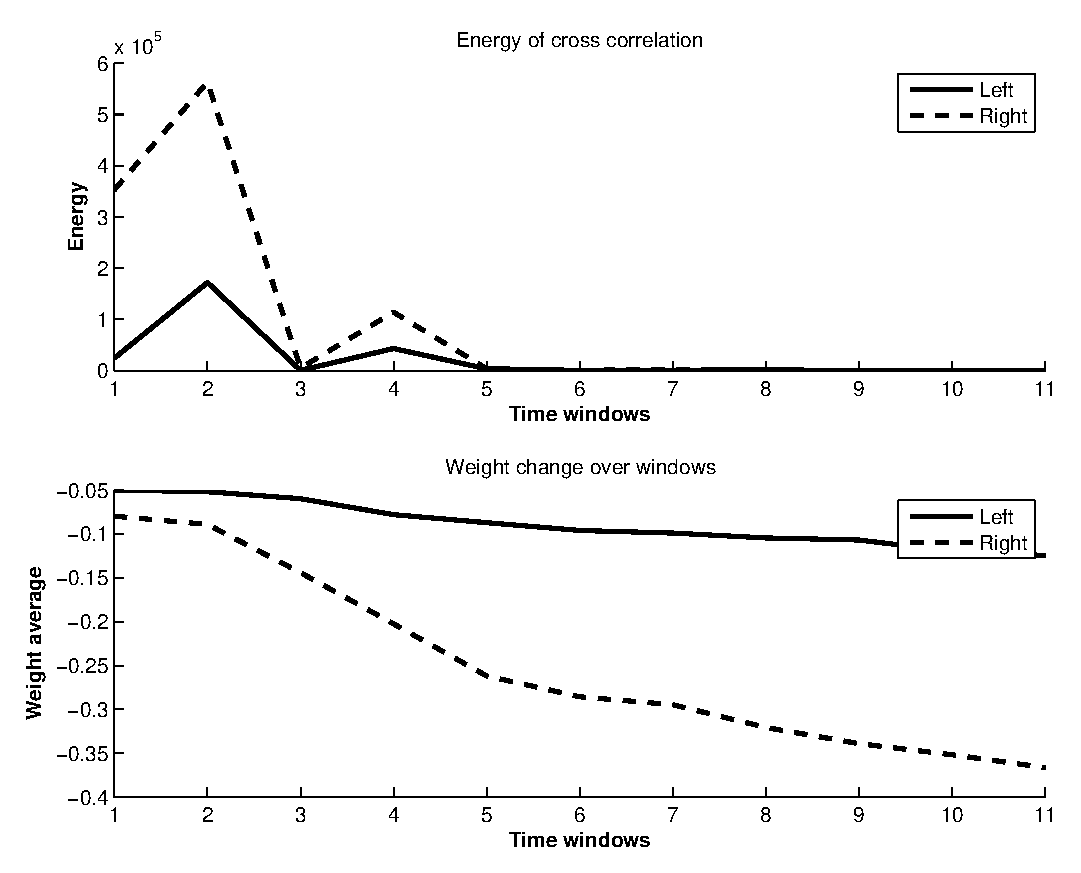
\includegraphics[scale=0.3]{figures/infomeasure/N2/power_xcorr_N=1_w=600.eps}}
    \caption[Max correlation for two learning agents]{Information measure analysis for $N=2$ agents
	      and $M=2$ obstacles computed in $k=1,...,11$ time windows.
	      Learning is switched on for all agents when ($k>1$). \label{fig:N2M2}}
  \end{center}
\end{figure}

\paragraph{Experiment with 4 agents and 2 obstacles}
The same considerations apply to the case of 4 agents with 2 obstacles.
Figs.\ref{fig:N4M2a} shows the measures for the first group of 2 agents and Fig.\ref{fig:N4M2b}
shows the measures for the second group of 2 agents.

\begin{figure}[htbp]
  \begin{center}
      \subfigure[Cross correlation maximum $M(c_{d}(k))$ when $N=4$ agents and $M=2$ obstacles for left (straight) and right (dashed) synapses. Measures from agent 0.]{
	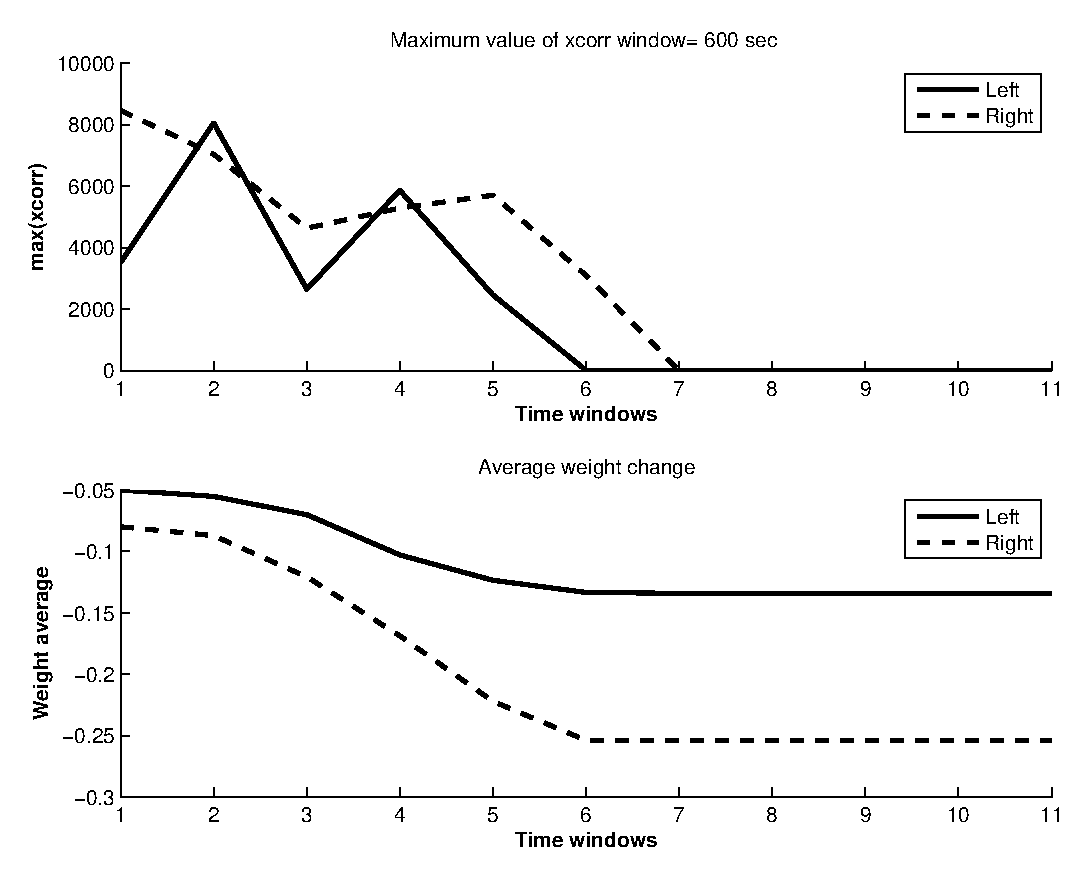
\includegraphics[scale=0.3]{figures/infomeasure/N4/maxcorr_N=0_w=600.eps}}
	\hspace{1pt}
      \subfigure[Energy $E(xcorr_{d}(k))$ when $N=4$ agents and $M=2$ obstacles for left (straight) and right (dashed) synapses. Measures from the agent 0.]{
	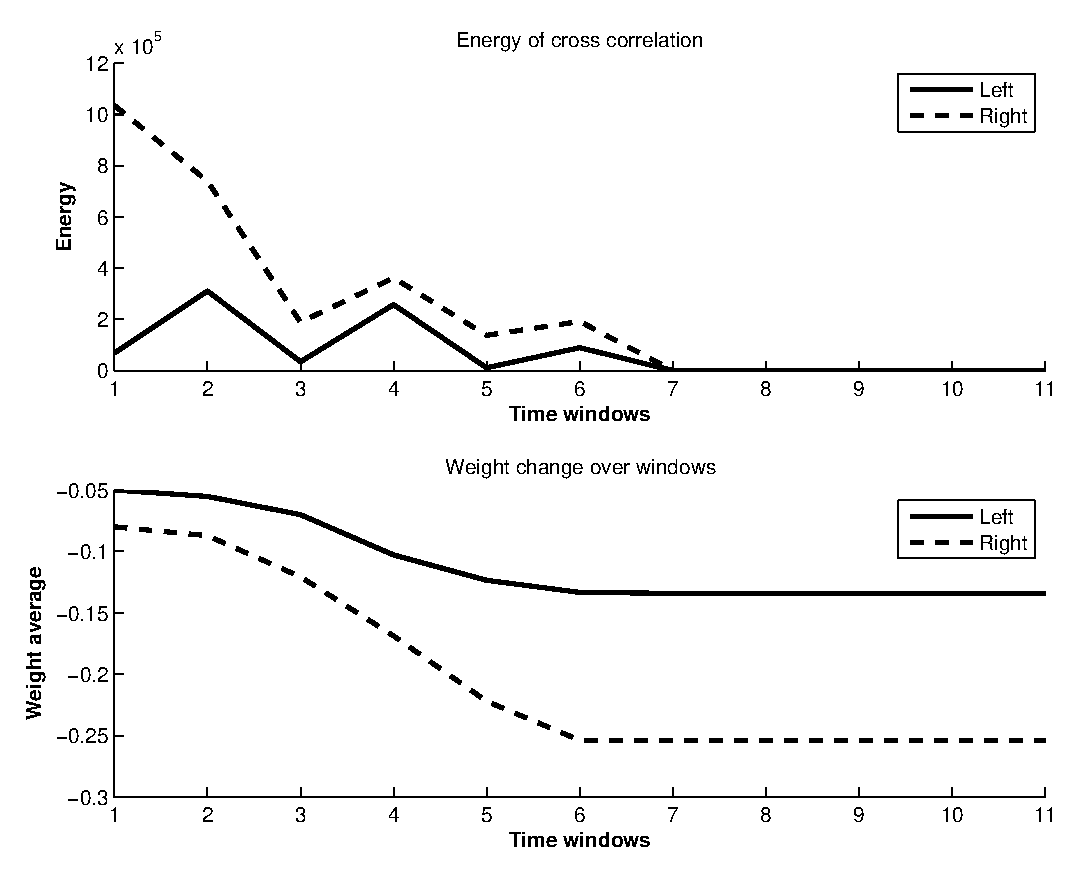
\includegraphics[scale=0.3]{figures/infomeasure/N4/power_xcorr_N=0_w=600.eps}}
\subfigure[Cross correlation maximum $M(c_{d}(k))$ for left (straight) and right (dashed) synapses. Measures from agent 1.]{
	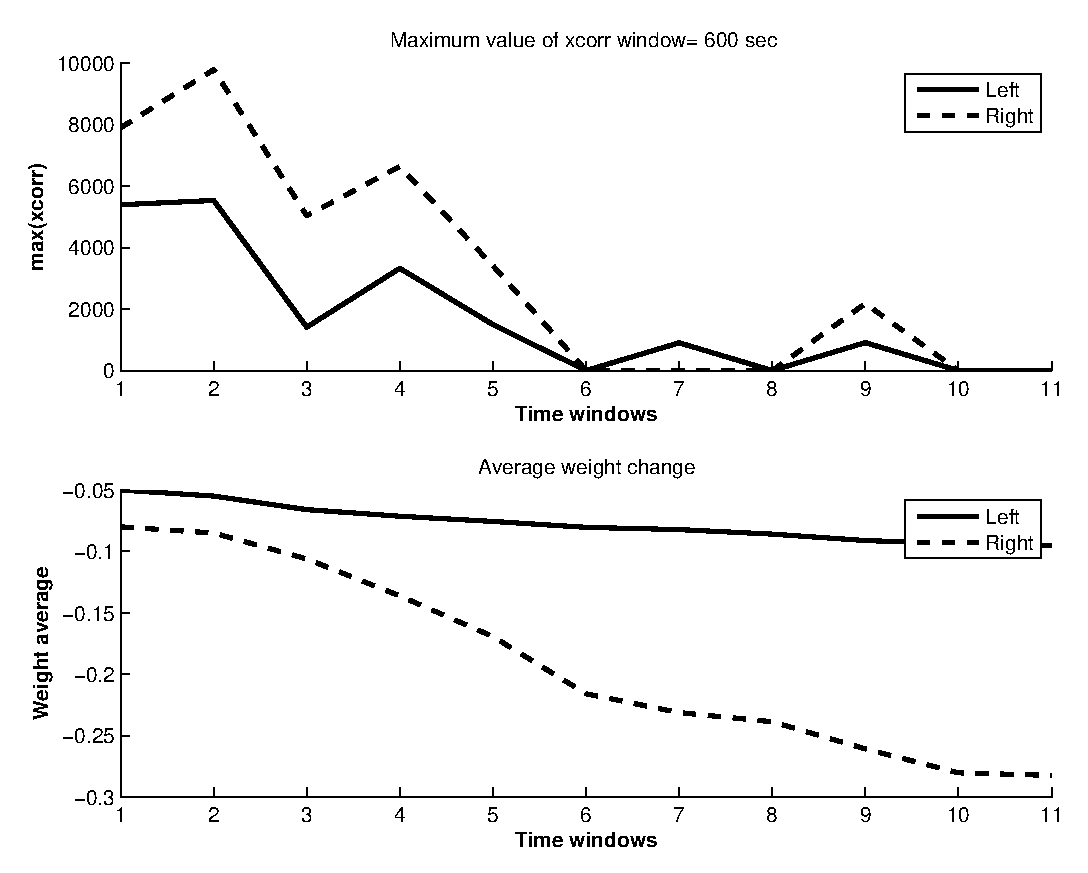
\includegraphics[scale=0.3]{figures/infomeasure/N4/maxcorr_N=1_w=600.eps}}
	\hspace{1pt}
      \subfigure[Energy $E(xcorr_{d}(k))$ for left (straight) and right (dashed) synapses. Measures from the agent 1. Learning starts after the first window.\label{fig:energylong}]{
	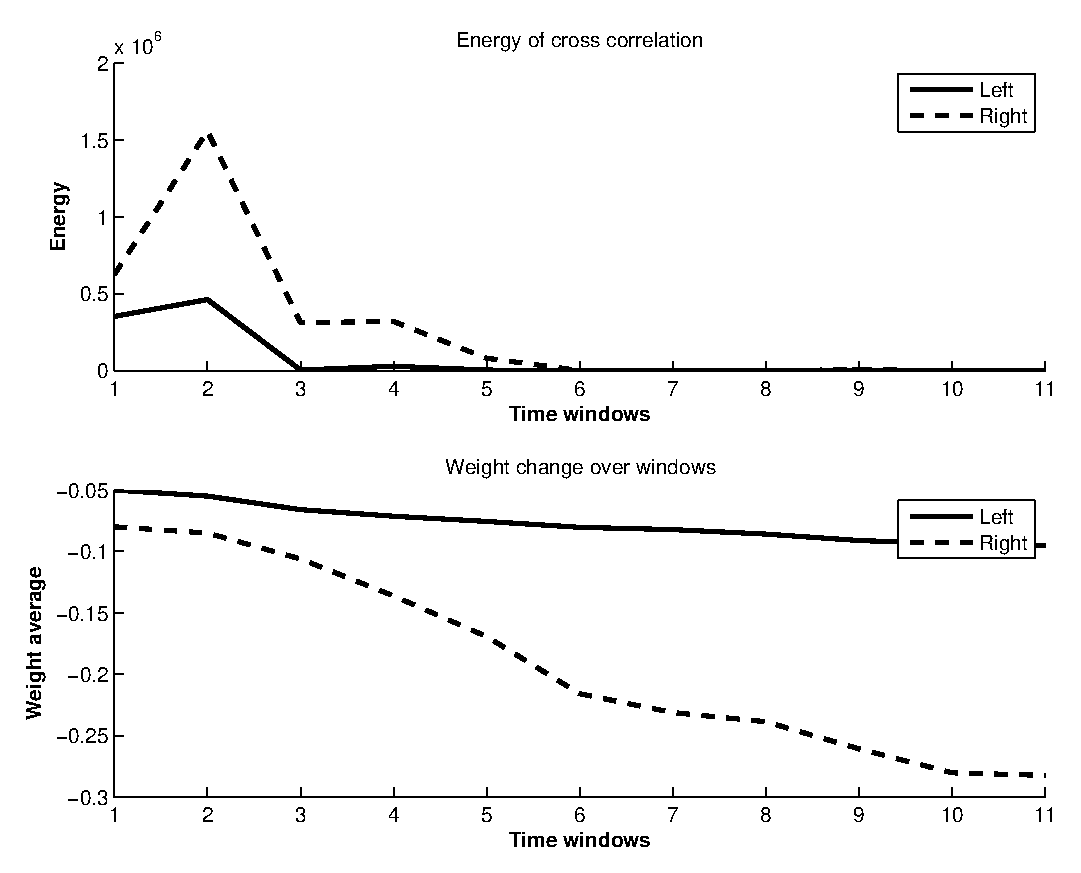
\includegraphics[scale=0.3]{figures/infomeasure/N4/power_xcorr_N=1_w=600.eps}}
    \caption[Max correlation for 4 learning agents A]{
      Information measure analysis for $N=4$ agents and $M=2$ obstacles computed
      in $k=1,...,11$ time windows. Learning is switched on for all agents
      when ($k>1$).\label{fig:N4M2a}}
  \end{center}
\end{figure}


\begin{figure}[htbp]
  \begin{center}
\subfigure[Cross correlation maximum $M(c_{d}(k))$ for left (straight) and right (dashed) synapses. Measures from agent 2.\label{fig:eqlearning}]{
	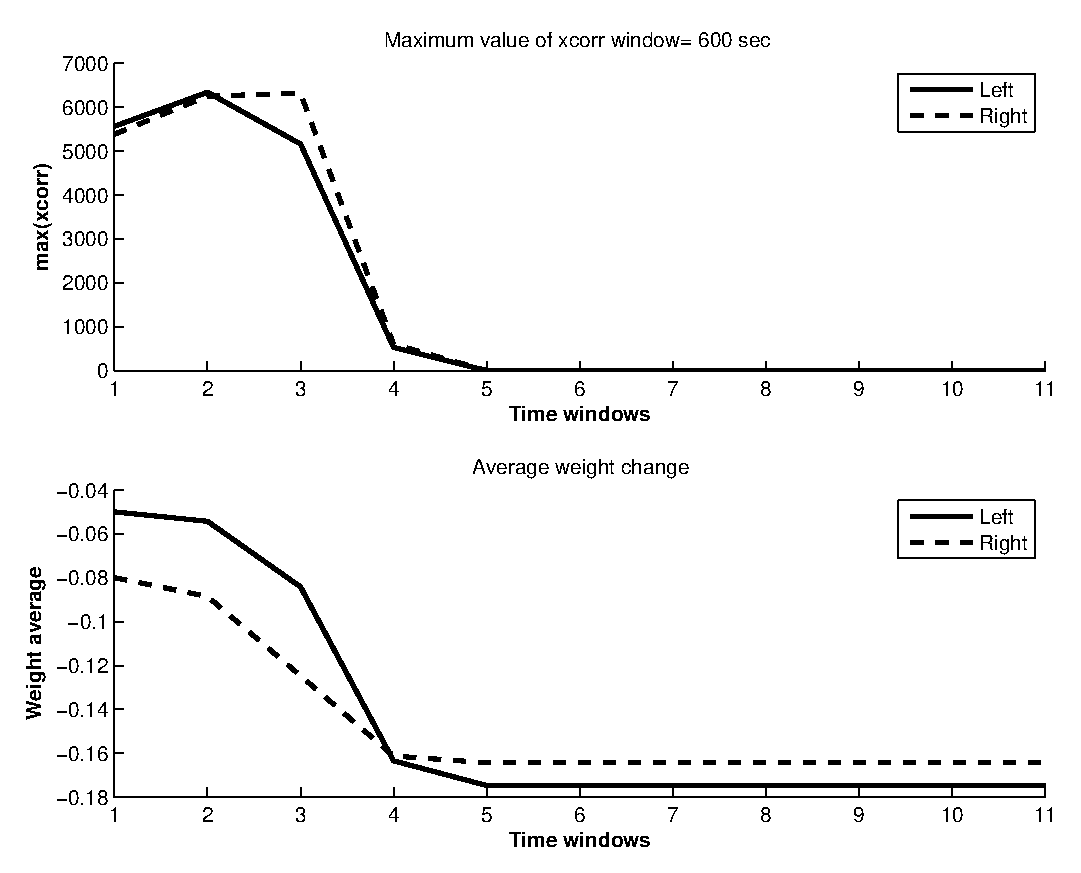
\includegraphics[scale=0.3]{figures/infomeasure/N4/maxcorr_N=2_w=600.eps}}
	\hspace{1pt}
      \subfigure[Energy $E(xcorr_{d}(k))$ left (straight) and right (dashed) synapses. Measures from the agent 2.\label{fig:energypeak} ]{
	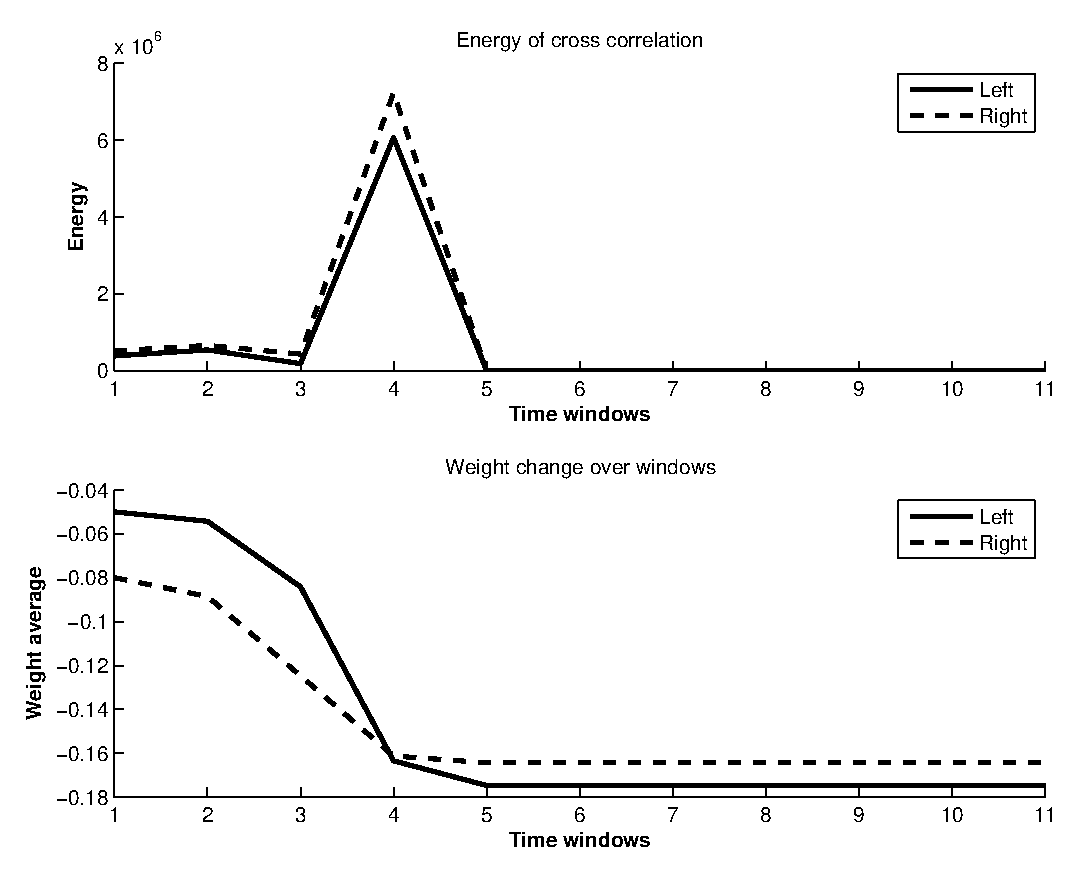
\includegraphics[scale=0.3]{figures/infomeasure/N4/power_xcorr_N=2_w=600.eps}}
\subfigure[Cross correlation maximum $M(c_{d}(k))$ for left (straight) and right (dashed) synapses. Measures from agent 3.]{
	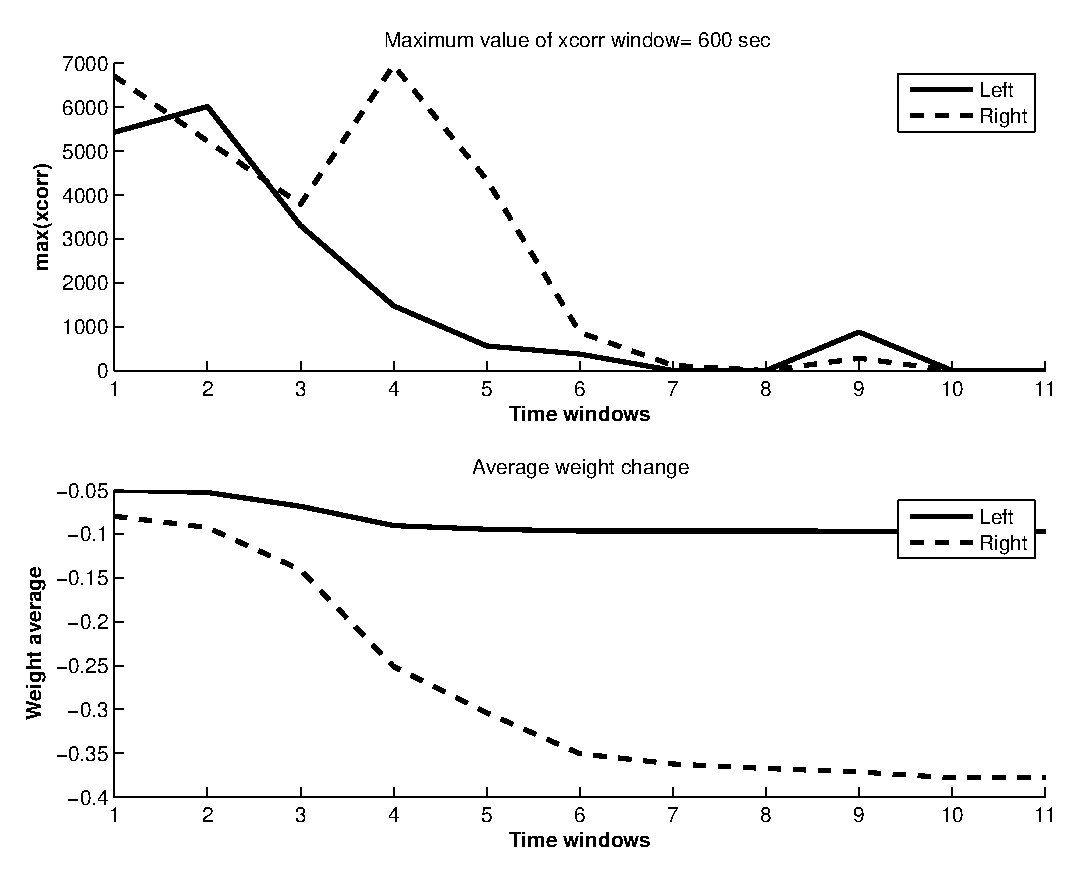
\includegraphics[scale=0.3]{figures/infomeasure/N4/maxcorr_N=3_w=600.eps}}
	\hspace{1pt}
      \subfigure[Energy $E(xcorr_{d}(k))$ for left (straight) and right (dashed) synapses. Measures from the agent 3.\label{fig:energylong2}]{
	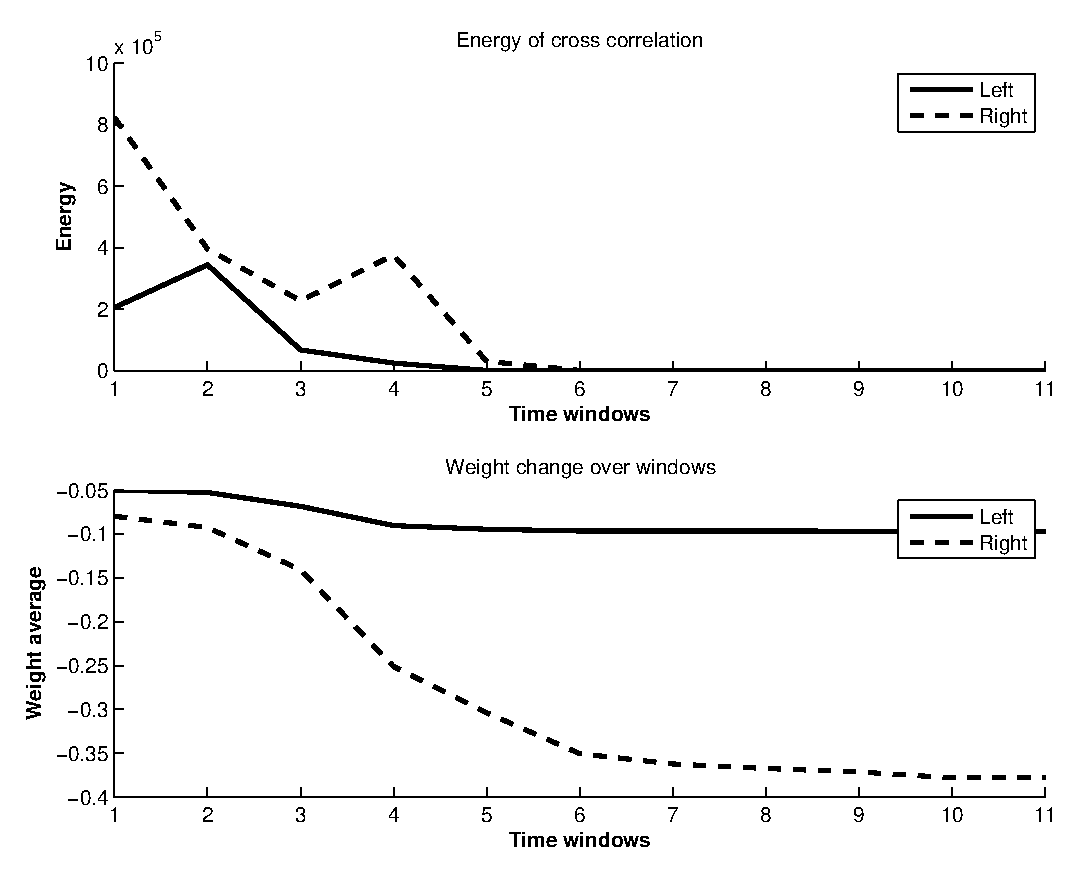
\includegraphics[scale=0.3]{figures/infomeasure/N4/power_xcorr_N=3_w=600.eps}}
    \caption[Max correlation for 4 learning agents B]{
	Information measure analysis for $N=4$ agents and $M=2$ obstacles computed
	in $k=1,...,11$ time windows. Learning is switched on for all agents
	when ($k>1$). \label{fig:N4M2b}}
  \end{center}
\end{figure}

As with the previous case the maximum cross correlations of each agent go
to zero when the learning is stable.
For example agent 2 in Fig.\ref{fig:N4M2a}(a,b) stabilises his learning weights
after $k>6$ time windows.
Comparing the maximum of the cross correlation for left and right synapses for all cases,
on average it occurs that $M(xcorr_{left}(k))>M(xcorr_{right}(k))$,$\forall k$:
agents learn more to use the left synapse which therefore is more responsible for the motor
behaviour. As a result the left synapse is more exposed to obstacle signals.
Instead the agent in Fig.\ref{fig:eqlearning} learns equally with both synapses
and in this case $M(xcorr_{left}(k))\cong M(xcorr_{right}(k))$.

An interesting property of the energy $E(xcorr_{d}(k))$ is that in all cases it tends
to zero $E(xcorr_{d}(k)) \cong 0$ when the weight change is stable $Avg(W_{predict,d},k) \cong 0$.
But there are exceptions like cases in Fig.\ref{fig:energylong},\ref{fig:energylong2}
where $E(xcorr_{d}(k)) \cong 0$ for $k>5$ even if the agent is still slowly learning.
This is due to the fine tuning that happens after the initial learning step, essentially
there are still some minor weak collisions which adjust the weights by a small factor.

The energy values can be used to for example agent 2 has a peak in the energy value
as in Fig.\ref{fig:energypeak} because there was an great learning experience at $k=4$,
where the weights' values jumped from $-0.08$ to $-0.18$.
Because the energy value calculates the density of collision events, it can be used
to verify the learning speed of the weight development.

\paragraph{Adding one agent}
When one more agent is added in the simulation at the time window $k=6 s$,
the other agents are ``surprised'' by its behaviour thus they need to adjust their weights.
I am investigating to what extent this behaviour can constitute a sort of primitive social teaching:
if there are some experienced robots the new ones do not have to learn a lot because the others are
compensating for their mistakes.
I can make a hypothesis that there is a critical mass of new agents
when the new ones need to start to learn as well.
The reader must remember that this model is not based on knowledge transfer models of
social colonies: the agents are not learning by imitation.
Learning by imitation requires rather complex functions which are not present in
simple organisms or agents like the one used in this simulation.

% % the energy signal has a peak for every agent: energy is an index of the ``surprise'' or novelty of new signals.
% The new inexperienced agents will be aided by the others to learn: their mates are already good in avoiding so
% for them will it be easier to learn. it is interesting to note that they learn less than others in the same time
% window: this effect is a feature of collaborative colonies where new members are facilitated by the experienced ones.
Fig. \ref{info:agentadd} shows the $M(xcorr_{left}(k)),M(xcorr_{right}(k))$ values
for an experienced agent.
When the new agent is dropped in the arena at time window 6, the agent sees it
by a peak in the cross correlation and thus needs to adjust its weights.  
\begin{figure}[htbp]
  \begin{center}
    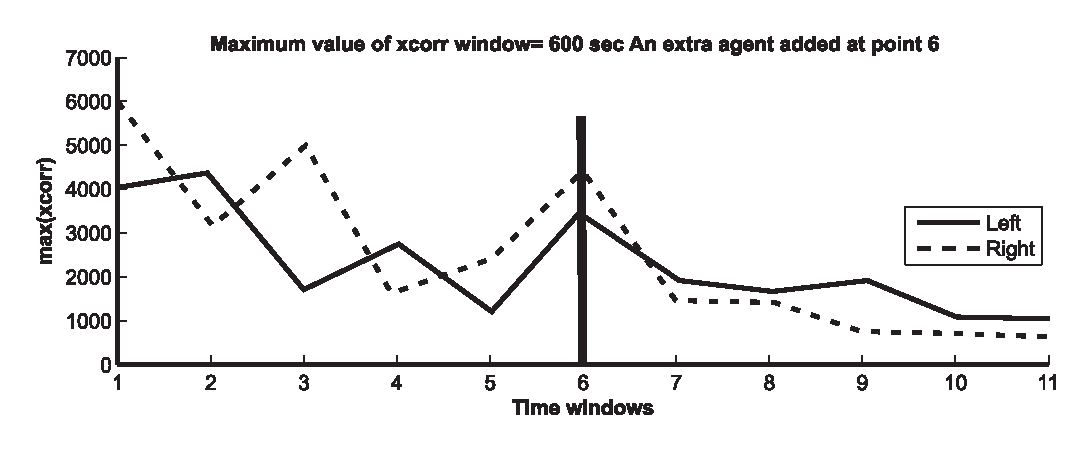
\includegraphics[scale=0.65]{figures/infomeasure/agentvariation.eps}
    \caption[Max correlation variation analysis]{A new agent is introduced
	    for t=6, the other agents needs to adjust their weights to the new
	    ``unpredictable'' friend.\label{info:agentadd}}
  \end{center}
\end{figure}
Unfortunately I did not have any more time to carry extensive analysis, but 
it would have been interesting how the performance of newly introduced agents is affected
by the other experience agents.
Probably the newly introduced agents wouldn't require a lot of learning as the
others are already successfully avoiding.

\subsection{Results: simple case results}
In this simple case there are 2 agents navigating in a rectangular space with
a number of 2 obstacles that are placed randomly in the environment (see Appendix \ref{Appendix:simplesocialsim}). 
Every simulation is run for $T=30$ minutes with a time step of $\varDelta=0.01s$,
the window for the correlation is $W=10$ seconds, therefore $cc(t)$ is computed
for $t=1,2,...,180$.

Anticipatory information is averaged over 100 simulations:
every simulation is randomised in terms of the robots' and obstacles' initial positions.
In the first time window the learning of the agents is switched off and $cc(0)\simeq 0.7071$
because the reflex of the agent is already preventing a full force impact, whereas for
$cc(t>0) \leq 0.7071$ because the impact of the collision can only be equal or decreased.

Fig.\ref{avoidance:resume}(B) shows that AI increases and stabilises to 6 bits when agents
have learned successfully: they are using 6 bits in the predictive loop to reduce the reflex.
Instead non learning agents are not using any bit to reduce the reflex.
The noise visible in Fig.\ref{avoidance:resume} is due to the random repositioning of the
obstacles and random collisions. In a perfect world if agents were able to avoid
perfectly $cc(t)\simeq 0$ and so $AI(t)\rightarrow \infty$.

\begin{figure}[htbp]
\begin{center}
\includegraphics[width=0.6 \textwidth]{infomeasure/simple/infoapplication.eps}
\end{center}
\caption[Max correlation application to a simplified case]{
\textbf{A)} Two agents are learning to avoid obstacles in a closed rectangular world.
At the very left the agent is only reacting to the obstacle thus $AI\simeq0$,
at the very right the agent has learnt successfully how to exploit the predictive
signal $u_1$ to avoid the contact thus $AI > 0$. 
\textbf{B)}  Anticipatory information computed for 2 learning agents.
When learning is stable it reaches a baseline level, $AI(t)\simeq 6$ bits.
If agents are not learning the anticipatory information is low $AI(t)\simeq 0.5$
bits, because $cc(0)\simeq 0.7071$. \label{avoidance:resume}}
\end{figure}

\subsection{Results: simplified social model results}
I apply now the \textbf{AI measure} to a social system such as the one published
in \citet{DiProdiMultiAgent} and described in section \ref{Chapter4:Social adaptation}
where a social system whose task is cooperative food foraging.
As for the avoidance case the agents learn how to use the distal sensors to
approach food (to increase their energy) or other agents (to get their energy).
Agents can forage directly from the food patches (see Fig.\ref{social:learning1}(B))
or reduce the energy of other agents who have previously got food (see Fig.\ref{social:learning1}(D)) .

Thus every agent has two competitive signals:
one from the food patches and one indicating the energy level of the other agents.
Indeed when antennas are in contact with another agent with high energy they produce
impulses on $x_{1,e}$ for far contacts and on $x_{0,e}$ for near contacts,
whereas when they are in contact with a food patch they produce impulses on $x_{1,f}$
for far contacts and on $x_{0,f}$ for near contacts.

Therefore the agent has 2 learning weights $\omega_{1,e}$ for energy and $\omega_{1,f}$
for food that both contribute to the motor output. When the simulation starts,
all agents have $\omega_{1,e}=\omega_{1,f}$ and therefore they approach any object because
according to the situation they will choose the food or the nearby agent.
Nevertheless during the simulation some agents (the seekers) will become more
attracted by the food  $\omega_{1,e}<\omega_{1,f}$, while the others (the parasites)
will become more attracted by the other agents with energy $\omega_{1,e}>\omega_{1,f}$.
An agent changes class or behaviour when the weights are swapped 
i.e. a seeker $\omega_{1,e}<\omega_{1,f}$ becomes a parasite $\omega_{1,e}>\omega_{1,f}$
(or viceversa) thus contributing to the system instability.

The bar diagram of Fig.\ref{social:learning1}(E) shows for every time window how
many times this swap has happened.The system self-stabilises to a number of seekers
and parasites whose number depends on the available resources:
in this case with 4 food resources there are 6 parasites and 4 seekers.
With more resources e.g. 10, there will be 6 seekers and 4 parasites.

Luhmann theorised that sub-systems are formed to reduce the complexity of the perceived environment:
in this case this means that agents are discarding part of the closed loop information.
This process is shown in Fig.\ref{social:learning1} by computing $AI$ for the energy and for the food signal.
The $AI(u_{1,e},u_{0,e})=AI_{energy}$ represents the anticipatory information for the energy attraction and the $AI(u_{1,f},u_{0,f})=AI_{food}$ for the food attraction.
For seekers the $AI_{food}>AI_{energy}$ increases as the system differentiates and conversely for the parasites $AI_{energy}>AI_{food}$.
In term of information it means that seekers are using $AI_{food}-AI_{energy}=2$ bits more to reduce the energy signal, whereas parasites are using $AI_{energy}-AI_{food}=2$ bits more to reduce the food.
\begin{figure}[!htbp]
\begin{center}
\includegraphics[width=0.8 \textwidth]{figures/infomeasure/simple/socialmeasure.eps}
\end{center}
\caption[Max correlation and learning in the simplified case]{B) A parasite is an agent that prefers an energy signal to a food one.  D) A seeker is an agent that prefers a food signal to an energy one produced by another agent. B) For parasites the anticipatory information for food is less than that one of the energy. C) For seekers the anticipatory information for energy is less than that one of
the food. E) There are a total of $N=10$ agents of whom 6 turn into parasites, and 4 turn into seekers after 20 time steps. The system stabilisation is a function of time: at the very
beginning agents are using both signals and their behaviour is unpredictable because they are switching between the 2 competitive behaviours.
After 20 time windows the agents have a more predictable behaviour resulting by the selection of the information. Minor oscillations are again
due to the noise resulting from the interaction between learning agents.\label{social:learning1}}

\end{figure}


\subsection{Results: differentiation and information measure}
I then computed the information measure $xcorr(k)$ in the same social model \citep{DiProdiMultiAgent}.
The results were compatible again with Luhmann's theory of information reduction
and social differentiation.
The Fig.\ref{info:social} is the outcome of computing the information on a
group of $N=10$ robots and $M=2$ food places.
There are 6 parasites and 4 seekers. In Fig.\ref{info:social} (A) for the 4 seekers
 the information measure of the food's signal is smaller than the average information
 measure of the agent signals. This means that the seekers learn to use only one
signal out of two in order to simplify the closed loop model.
In Fig.\ref{info:social} (B) for the 6 parasites the information measure of the
 agents' signal is smaller than the average information measure of the food's signals.
This means that the parasites learn to use only one signal out of two in order to
 simplify the closed loop model. As I expected when the system is not stable
 Fig.\ref{info:social} (C)  -the agents are switching their class-
the information measure for the food signals and the agent signals are
crossing each other, but when the system becomes stable - switching rate is
approaching 0- I can see that the two information measures start to separate.

\begin{figure}[htbp]
  \begin{center}
    \includegraphics[scale=0.5]{figures/infomeasure/LearningDifferentiation.eps}
    \caption[Max corr computed on the social system]{The information measure computed
      on a group of $N=10$ robots. (A) information measure computed on the 4 seekers
      and compared to the average measure of the 6 parasites. (B) information measure
      computed on the 6 parasites and compared to the average measure of the 4 seekers.
      (C) The switching rate: how many agents changes their class for every time window.
      The system is stable when the switching rate is 0, in this case after 7 windows.
      \label{info:social}}
  \end{center}
\end{figure}

Luhmann theorised that in society, specialised groups emerge when they reduce
the uncertainty of the environment-system boundary in a recursive process.
The model's results validate his theory because agents are selecting to use one
information rather than the other one to simplify the model of the environment's loop.

\subsection{Discussion}
Devising a measure of information for learning agents in a closed loop is a challenging task.
Previous approaches in the literature are all based on the concept of Shannon's
entropy applied to adaptive controllers.
There are 3 main problems in using Shannon's entropy:
\begin{itemize}
 \item it ignores semantics when dealing with transmitted data: when a sequence of
symbol is transmitted, every symbol carries the same importance, only their probability
 of occurrence plays a role in Shannon's model.
\item is not suitable for closed loop: joint and disjoint probabilities change continuously
 in the closed loop and therefore they must be estimated continuously.
\item probability encoding discards temporal information: positive and negative phase
 delay induces the same variation in the mutual information measure (see Appendix A).
\end{itemize}
\citet{PhysRevLett.84.1156} consider the perception action-loop
 in terms of a communication channel-like model.
Also \citet{organizationInfo} recently has been using the
same approach: the perception-action loop enables an agent to use its actuators
as a channel to transmit information into the environment.
The information can later be acquired from the environment by the same agent or other agents.
 In our measure there is no such transfer channel: temporal information
relevant to the agent is computed only at the inputs which contains the feedback
 of the outputs. It is simple and easy to compute and it does not require the modelling of the agent's
 controller as an information channel.
Recently, \citet{shannonSemantic} has been working on evolving sensors and has
 introduced an operational notion of Shannon-type quantification of relevant information:
\begin{itemize}
 \item it quantifies relevance with respect to a given agent or decision system.
 \item it yields a measure for the usefulness of sensors or about an agent's state
of knowledge with respect to a POMDP (partial observable markov decision process)
\end{itemize}
The problem of this approach is that it requires a discrete formulation of
an agent, and its application to a general controller is not possible.
The limit of the \textbf{maxcorr} measure is that it is dependent on the particular implementation
of our controller and cannot be applied to other adaptive algorithms unless
they are based on a similar temporal input structure.
The limit of the \textbf{AI measure} is that although it quantifies the learning
behaviour in terms of bits, it does not provide an axiomatic framework and
thus can be mathematically weak.
Therefore in Section \ref{Chapter6:Information Flow}, the author developed a more
advanced measure based on the concept of information flow which is inspired by the
work of \citet{LungarellaInformation}.


